\subsection{Battery Data for training and validation} \label{subsec:b_data}
% Battery data description and overview. **Table III**
%
Model training was conducted over a lithium-ion battery's cycling data obtained by the Battery Research Group of the Center for Advanced Life Cycle Engineering (CALCE) Group at the University of Maryland~\cite{noauthor_calce_2017} in 2012.
According to the associated paper, the battery cycling was performed with a BT2000 tester machine, manufactured by Arbin Instruments, Texas, USA, and controlled with official Arbin Mits Pro Software (v4.27)~\cite{xing_state_2014}.
% \textcolor{red}{\textbf{The value of charge has not matched with battery testing of the similar cells conducted during this research with freshly bought M1-B series cells.
% Despite their small difference, the CALCE most likely used a series of two cells with either doubled current or 1000 cycles used batteries before publishing the data with reduced capacity.}}
Table~\ref{tab:battery} highlights selected battery characteristics directly from the datasheet~\cite{noauthor_anr26650m1a}.
\ifthenelse{\boolean{thesis}}{
\begin{table}[ht]
    \renewcommand{\arraystretch}{1.3}
    \caption{Battery characteristics}
    \centering
    \label{tab:battery}
    \begin{tabular}{ l c c c c c }
        \hline\hline \\[-3mm]
        Brand & Cell      & Cell & Battery & Nominal          & Charge/discharge\\
        name  & Chemistry & Type & Weight  & Capacity $C_{N}$ & cut-off voltage \\
        % \makecell{Brand name} & \makecell{Cell Chemistry} & \makecell{Cell Type} & \makecell{Battery Weight} & \makecell{Nominal Capacity $C_{N}$} & \makecell{Nominal Voltage} & \makecell{Charge/discharge cut-off voltage} \\
        \hline
        %A456 \\ (former A123) & 76g+-1g & 2.3Ah & 3.2V & 3.65V, 2.0 V\\
        A123   & LiFePO4 & ANR26650 & 70g        & 2.3Ah & 3.6V\\
        (2012) &         & \textbf{M1-A}     & \textpm 2g &       & 2.0V \\
        \hline\hline
    \end{tabular}
\end{table}
} {
    \begin{table}[H]
        \caption{Battery characteristics.}
        % \centering
        \label{tab:battery}
        \begin{adjustwidth}{-\extralength}{0cm}
        %\centering %% If there is a figure in wide page, please release command \centering
        \begin{tabularx}{\fulllength}{CCCCCC}
            \toprule
            \textbf{Brand Name} & \textbf{Cell Chemistry} & \textbf{Cell Type} & \textbf{Battery Weight} & \textbf{Nominal} & \textbf{Charge/Discharge Cut-Off Voltage} \\
            \midrule
            A123 & $LiFePO_4$ & ANR26650 & 70 g   & 2.3~Ah & 3.6~V\\
            (2012) &    & M1-A  & \textpm 2 g &   & 2.0~V \\
            \bottomrule
        \end{tabularx}
        \end{adjustwidth}
    \end{table}
}

% How to work with battery data and which were selected.
%
The battery cycling data over 2 Li-ion cells were stored as Excel spreadsheets over the temperature range 0 \textdegree{}C to 50 \textdegree{}C degrees, with 10 degree steps and a tolerance of around 0.5--1 \textdegree{}C, including an ambient temperature of 25 \textdegree{}C.
Each testing cycle contained three profiles, distinguished by their current consumption, emulating a stress test or driving scenarios: dynamic stress test (DST)---Figure~\ref{fig:current-profs}a, highway (US06)---Figure~\ref{fig:current-profs}b and the federal urban driving schedules (FUDS)---Figure~\ref{fig:current-profs}c.
Each cycle consisted of charge and discharge periods, with a sampling rate of 4 Hz and 1 Hz, respectively.
Charging periods were linearly interpolated to match the data sampling rate.
%without additional random noise due to insignificant impact.
The range of 20 \textdegree{}C to 50 \textdegree{}C was used as a training and validation dataset, since this was the most common temperature range for the EVs involved in this research.
This resulted in $\sim$58,613 and $\sim$12,171 samples for training and validation over one profile.
Each model from \mbox{Table~\ref{tab:experiment}} was trained independently on each drive cycle profile and then tested against the other two, as per Mamo and Wang~\cite{mamo_long_2020}.
The performance calculation was conducted over two cycles of 30 \textdegree{}C and 40 \textdegree{}C samples for each of the two remaining profiles, leading to a total of 47,022 testing samples.
% After compleating three models per profile for every evaluated method, the overall performance calculation has been conducted against all samples of all three profiles, making a good performance capture for any possible driving conditions.

% State of charge calculation with equations.
%
As in any battery usage scenario, the state of charge was provided in the CALCE data.
However, the Arbin machine stored both in and out charges as separate arrays, along with the applied current.
The SoC value could be calculated from the difference between charge and discharge capacities in Ah.
% The \textit{MinMax} algorithm allows adjustment of the minimum and maximum point of the SoC to be within bounds 0 and 100\%.
% \begin{equation}
%     \begin{split}
%         \hat{SoC} &= MinMax(C-D)
%         \label{eq:SoC-DC}
%     \end{split}
% \end{equation}
The resulting trend could be validated with Coulomb counting, using the integral of the consumed and/or produced current $I$ between initial $t_0$ and the end of cycle $t_n$ time, divided by the (converted to seconds) nominal capacity $C_{N}$ of the batteries, as per \mbox{Equation~(\ref{eq:SoC-calc})}.
\begin{equation}
    \begin{split}
        \hat{SoC} &= \frac{\int_{t_0}^{t_n} I(t)dt} {C_{N}} = \frac{\int_{t_0}^{t_n} I(t)dt} {(2.3*3600)} \\
        \label{eq:SoC-calc}
    \end{split}
\end{equation}
\vspace{-16pt}

The final expected value was rounded to two decimal places in all scenarios to simplify the training and testing processes.
% , as per Equation~\ref{eq:SoC-round}.
% \begin{equation}
%     \begin{split}
%         SoC &= \frac{int(100\times\hat{SoC})}{100}
%         \label{eq:SoC-round}
%     \end{split}
% \end{equation}
%! Elaborate that at different temperatures, which produces above 100%
% Optionally, all calculated SoC can be adjusted using \textit{MinMax} scaler algorithm to set bounds between 0-100\%, \mbox{Equation~\ref{eq:MinMax}}.
% \begin{equation}
%     \begin{split}
%         SoC_{0\%} + \frac{ \left(SoC - \min \left( SoC \right)\right) \left( SoC_{100\%} - SoC_{0\%} \right) }
%                          { \max \left( SoC \right) - \min \left( SoC \right)} \\
%     \end{split}
%     \label{eq:MinMax}
% \end{equation}

%%%% The methodology unification with other authors will not be used in the current research since the quality and age of the tested batteries cannot be verified.
\begin{figure}[H] %Attention AE: please ensure there is a space before the parentheses containing the units.
    \begin{subfigure}[b]{0.45\textwidth}
        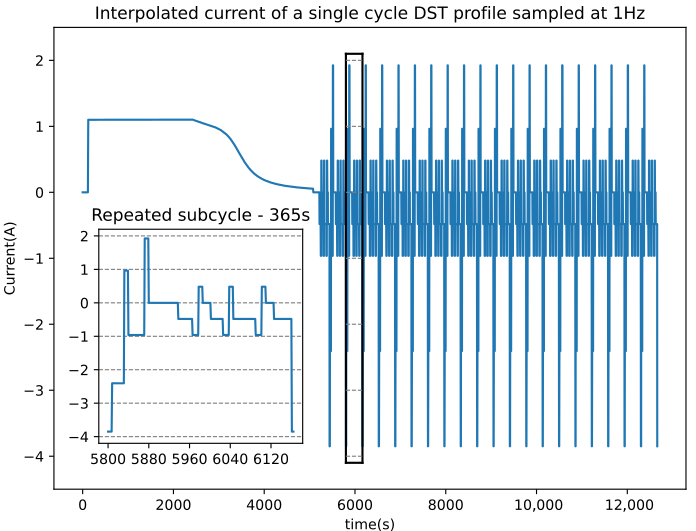
\includegraphics[width=6cm]{II_Body/images/Current-DST.png}
        \caption{\centering}
        \label{subfig:profs-DST}
    \end{subfigure}
    \vspace{1pc}
    \begin{subfigure}[b]{0.45\textwidth}
        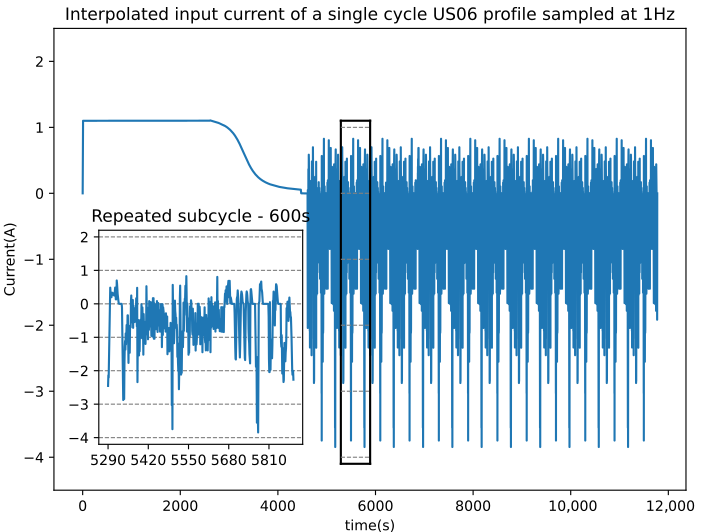
\includegraphics[width=6cm]{II_Body/images/Current-US06.png}
        \caption{\centering}
        \label{subfig:profs-US}
    \end{subfigure}
    \vspace{1pc}
    \begin{subfigure}[b]{0.45\textwidth}
        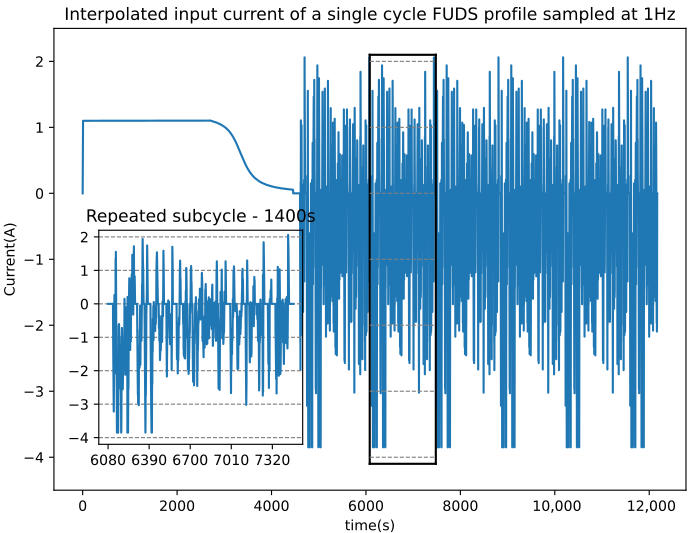
\includegraphics[width=6cm]{II_Body/images/Current-FUDS.png}
        \caption{\centering}
        \label{subfig:profs-FUDS}
    \end{subfigure}    
    %   \caption{\hl{Cell} %MDPI: please consider adding the descriptions for subfigures a--c in the main figure caption aswell. Please use commas to separate thousands for numbers with five or more digits (not for four digits) in the picture. e.g., "10000" should be "10,000
    %  Current
    %  of three battery testing profiles, emulating Constant-Current-Constant-Voltage charge and regenerative discharge until cells reached top or bottom cut-offs.}
    \caption{Cell current of three battery testing profiles, emulating a constant-current--constant-voltage charge and regenerative discharge until cells reached top or bottom cutoffs. (\textbf{a}) Dynamic stress test (DST) of 20 repeated subcycles; (\textbf{b}) highway driving schedule (US06) of 12 repeated subcycles; (\textbf{c})~federal urban driving schedule (FUDS) of 6 repeated subcycles.}
    \label{fig:current-profs}
\end{figure}
